As a conclusion of section \ref{sec:StateOfTheArt}, the current techniques cannot be used for tritium monitoring in quasi-real time since they have either a high LDL or they work in off-line method. 

To overcome these limitations the \textit{Tritium} project \cite{TRITIUM}, with the title of "Design, construction and commissioning of automatic stations for quasi-real time monitoring of low radioactive levels of tritium in water", was proposed.

The \textit{Tritium} collaboration is an international consortium of six different European institutions from three European countries: The University of Aveiro, in Portugal, The University of Bordeaux and The \textit{National Center for Scientific Research} (CNRS, Section Aquitaine-Limousin), in France and the University of Extremadura, The \textit{Junta de Extremadura} and The University of Valencia, in Spain.

This project was funded by the Interreg Sudoe program of the European Economical Community, EEC, in year 2016 call, with the reference number SOE1/P4/EO214. The purpose of this project is the development of an automatic station for in-water tritium monitoring, in situ and in quasi-real time. The tritium detector consists of a bunch of scintillating fibers in contact with the tritium water sample which are in charge of detecting the tritium decay electrons. These fibers are read out with several photosensors (photomultiplier tubs, PMTs, or silicon photomultiplier arrays, SiPM) in time coincidence. The specific efficiency obtained by Moghissi for scintillating fibers is sufficiently high to justify our choice of scintillating fibers as a detection medium. Additional elements are used to improve the tritium detection sensitivity such as a water purification system, which prepares the water sample before introducing it in the detector for tritium measurement and a cosmic veto and a pasive shielding, which reduces the natural radioactive background of the tritium detector. Several electronic modules which control the different parts of the monitor, analyze the tritium measurement and send an alarm if the configured limit ($100~\becquerel/\liter$) is exceeded.

A crucial problem is to distinguish tritium signals from the background because tritium events has low energy ($\sim~\keV$) and fall in an energy range of the spectrum where background events are significant . To reduce the background counts of TRITIUM monitor, coincidence techniques are employed.

%It is important to check the water tightness of each prototype because if the water reaches the photosensor it will be irreparably damaged. On top of that if we use high concentrations of tritium in water for laboratory tests we can contaminate this laboratory, which could be dangerous for the healthy of the workers and it could spoil measurements of future experiments.

The TRITIUM monitor will be installed in the Arrocampo dam, Almaraz (Spain), displayed in Figure \ref{fig:Arrocampo}, where the Almaraz NPP releases the water from its secundary cooling circuit. This NPP has two nuclear reactors of PWR type. Arrocampo dam is located near the Tagus river, shown in Figure \ref{subfig:TajusRiver}, which is the longest river in Spain, with a length of $1007~\kilo\meter$. This river, shown in Figure \ref{subfig:Arrocampo_Dam}, rises in Aragon (Spain) and flows into the atlantic Ocean, through Lisbon (Portugal). The water of this river is used for agriculture and drinking water by both Spanish and Portuguese people. For this reason, an international cooperation is necessary in order to control and maintain the quality of the tagus river water.

\begin{figure}
\centering
    \begin{subfigure}[b]{0.45\textwidth}
    \centering
    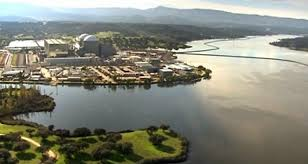
\includegraphics[width=\textwidth]{2Introduction/ArrocampoDam.jpeg}  
    \caption{\label{subfig:Arrocampo_Dam}}
    \end{subfigure}
    \hfill
    \begin{subfigure}[b]{0.45\textwidth}
    \centering
    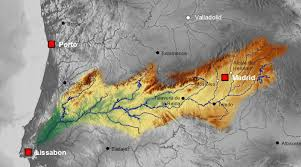
\includegraphics[width=\textwidth]{2Introduction/RioTajo.jpeg}  
    \caption{\label{subfig:TajusRiver}}
    \end{subfigure}
 \caption{(Above) Arrocampo dam and Almaraz Nuclear Power Plant. (Below) Tagus river along Spain and Portugal.}
 \label{fig:Arrocampo}
\end{figure}

Each institution of TRITIUM collaboration has focused its efforts in the development of a different part of this project:

\begin{enumerate}
\item{} The Extremadura group has developed and installed the water purification system to produce water with very low conductivity, $\sigma \approx 10~\mu\sievert/\cm$ (two orders of magnitude less than before the cleaning process, $1000~\mu\sievert/\cm$). This cleaning process is very important for two reasons. On the one hand, for maintaining the TRITIUM detector very clean, which is critical for its long-term functionality. On the other hand, to reduce the natural background since several natural radiactive isotopes present in this water (except tritium) are removed such as $\ce{^{222}Rn}$, $\ce{^{40}K}$ or $\ce{^{137}Cs}$. This system is explained in section \ref{sec:UltraPureWaterSystem}.

\item{} The French group has developed the pasive shielding for the detector. The shielding is made of radiopure lead with very low intrinsic activity in order to reduce the external natural background of the system. This shielding is presented in section \ref{subsec:SetUpPassiveShield}.

\item{} The Portuguese and Spanish groups have collaborated for designing, developing and building four different prototypes of the TRITIUM detector and active vetos for reducing cosmic events. These prototypes and vetos are explained in chapter \ref{chap:Prototypes} and section \ref{subsec:SetUpActiveShield} respectively. They have also carried out simulations of this system. These simulations are explained in chapter \ref{chap:Simulations}.

\end{enumerate}

The important characteristics of the TRITIUM detector must have are:

\begin{enumerate}

\item{} \textit{Compactness}. Compactness is an important requirement because in the place where the detector is planned to be installed, Arrocampo, there is little space. Compactness also allows portability and cost reduction.

\item{Modularity}. The modularity of the TRITIUM detector is important for its flexibility in the geometrical configuration and to improve its tritium detection sensitivity, which increase in a scalability way. Modularity also makes it easy its construction and maintenance..

\item{} \textit{Thin active volume and large active area}. The mean free path of the $\beta$ particle of tritium decay is very short so thin detector active volumes are needed. In practice, active thickness beyond the mean free path of the tritium electrons only contributes to background. In addition, as reported in section \ref{sec:StateOfTheArt}, the efficiency of this type of detector scales with the active area, so it is crucial to design the detector with the largest possible active area.

\item{} \textit{High efficiency detection for tritium}. As the tritium activities to be measured are very low, we cannot afford the loss of tritium events as it strongly affects the reliability of the tritium measurement..

\item{} \textit{High specificity to tritium}. The monitor has to be able to distinguish the tritium signal from the signal due to other radiactive elements present in the sample.

\item{} \textit{Quasi-real time response}. It is important that the system operates in quasi-real time ($1~\hour$ or less) in order to detect any anomalous tritium release as fast as possible. 

\item{} \textit{Ruggedness}. The final goal of the project is to install an automatic system working during a number of years requiring only scarce intervention of specialized operators. Therefore, a rugged monitor is required.

\end{enumerate}

In order to get the measurement in quasi-real time, it is needed to work \textit{in situ}, that is, in the same place where the water sample is taken. Working \textit{in situ} has some advantages such as: 1) Faster and cheaper maintenance, since the sampling process, chain of custody, etc. are eliminated, 2) Continuous measurements are carried out and 3) Safer monitoring since personal exposure dose is reduced, 4) Changes in activity levels can be detected quickly.


%In order to get the measurement in quasi-real time it is needed to work \textit{in situ}, that's, in the same place that the sample is taken. Working \textit{in situ} has some benefits:

%\begin{itemize}
%\item{} a faster monitor because we eliminates the process of taking the sample, the chain-of-custody until this sample arrive to this laboratory and the complexity which involve these tasks. 

%\item{} a better monitor since if we can work \textit{in site}, our measurements can be more frequent hence we will can identify cahnges in the activity earlier.

%\item{} a cheaper monitor because we have not only the material costs attached to the sample collection, chain-of-custody of this sample, shipping of this sample to the laboratory, etc. but we have also eliminated the costs attached to the specialized staff who are involving in these tasks. Our detector will only need frequent calibrations each time in order to ensure its correct operation.

%\item{} a safer monitor since the personal exposure dose is reduced and the changes in activity are detected fastly. On top of that we remove the possibles mistakes which can be done by specialized staff.

%\end{itemize} 